\section{État actuel du projet et prévision pour les prochaines soutenances}
        
        Voici un tableau d'avancement des tâches réalisé et de nos prévisions pour les prochaines soutenances : \\ \\
    
        {\normalsize
    	\begin{tabular}{|p{7cm}|p{2.4cm}|p{1.8cm}|p{1.8cm}|}
    		\hline
    		Tâches & Actuellement & \multicolumn{2}{|c|}{Soutenance} \\ 
    		\cline{3-4}
    		& & \no 2 & \no 3 \\
    		\hline
    		Système de fichier & 75\% & 100\% & 100\% \\
    		\hline
    		Sauvegarde & 40\% & 75\% & 100\% \\
    		\hline
    		Compression & 25\% & 60\% & 100\% \\
    		\hline
    		Chiffrement & 50\% & 80\% & 100\% \\
    		\hline
    		Site web & 35\% & 80\% & 100\% \\
    		\hline
    		Interface graphique & 25\% & 60\% & 100\% \\
    		\hline
    	\end{tabular}
    	\label{répartition}}

\newpage

\section{Sauvegarde}
    
    \subsection{Système de fichier}
        \paragraph*{}
        Pour cette soutenance, nous avons commencé le système de fichiers. Nous avons commencé par créer l'arbre représentant l'arborescence des fichiers. Ceci est nécessaire pour la restauration des fichiers mais aussi pour leur sauvegarde et la sauvegarde des différents états. Pour construire cet arbre, il nous a fallu parcourir toute l'arborescence d'un chemin donne.\\
        Pour cela, nous avons choisi d'utiliser la bibliothèque standard et \textit{dirent}. Parcourir un fichier ne s'est pas avéré très complique au début, nous avons même réussi a faire une fonction qui permet de copier-coller des dossiers très facilement lors de nos essais. Cependant, lors de la construction de l'arbre, plusieurs problèmes se sont posés. Tout d'abord, il faut gérer les cas de récursion (dossier dans un dossier) mais aussi les cas terminaux: fichiers ou dossiers vides.\\
        Pour toutes ces raisons, nous avons décidé d'implémenter ceci de manière récursive et de faire plusieurs fonctions. Nous avons donc une fonction qui crée l'arbre si c'est un fichier et une autre si c'est un dossier. Cependant, si c'est un dossier, il a fallu gérer le cas particulier du dossier vide. Pour cela nous avons une condition spéciale dans la fonction.\\
        \paragraph*{}
        Un autre problème est arrive ensuite. Sous Linux tout est fichier, y compris les dossiers. Nous avons donc du comprendre comment distinguer un dossier d'un autre fichier pour gérer nos appels correctement. Heureusement, les librairies standard contiennent déjà des éléments pour nous aider a gérer ceci.\\
        Ainsi, dans la fonction principale, nous faisons une première vérification du type de fichier. Si celui-ci est un fichier "simple", nous appelons la sous-fonction qui gère les fichiers et sinon, nous appelons la fonction qui gère les dossiers qui elle-même appelle récursivement la première ou elle-même.\\
        Le second problème majeur que nous avons rencontre est la présence des dossiers "." et ".." dans chaque répertoire. Ces deux dossiers représentent respectivement le dossier actuel et le dossier parent. Le problème de ces fichiers est qu'ils sont toujours présents et que si on appelle récursivement dessus, on s'expose a une récursion infinie, retournant en boucle dans le répertoire actuel ou dans les dossiers parents jusqu'au root, posant ainsi de potentiels problèmes d'autorisation.\\
        Afin d'éviter ce problème nous sommes forces de vérifier chaque appel pour ne pas appeler sur ces dossiers, sous peine de crash.\\
        \newpage
        \paragraph*{}
        \begin{lstlisting}[style=CStyle]
    struct meta_data
    {
        char *path;
        struct stat fs;
    }meta_data;
    
    struct meta_tree
    {
    struct meta_data *data;
    struct meta_tree *son;
    struct meta_tree *sibling;
    }meta_tree;
		\end{lstlisting}
		Ci-dessus se trouvent les structures utilisées pour stocker l'arborescence de fichiers. Pour le moment, les données stockées sont simples mais il est possible d'en rajouter de plus complexes, notamment la version etc...\\
		\paragraph*{}
		Une fois que l'arbre a été construit, il a fallu le sauvegarder et pour cela nous avons décidé de tout gérer nous même. La structure contenant des pointeurs, il est inutile de sauvegarder ceci puisque ce qu'ils représentent sera perdu entre temps. Il est plus intéressant de sauvegarder ce qu'ils représentent. Pour commencer, la sauvegarde a été découpée en sauvegarde des données, c'est a dire chemin et statistiques et en sauvegarde récursive.\\
		Pour sauvegarder les données, nous avons choisi de sauvegarder d'abord la longueur du chemin puis celui-ci et enfin les statistiques du fichier. Ceci a été fait afin de faciliter la restauration.\\
		Pour sauvegarder le reste de l'arbre, il a fallu sauvegarder un élément permettant de savoir si le noeud a un frère ou un fils afin de savoir si le prochain noeud sauvegarde est lie a l'actuel. Pour cela, nous avons décidé de sauvegarder ces deux informations dans un byte en créant des macros et en utilisant des opérations bitwise. Cela nous permet de simplifier la restauration.\\
            
    \subsection{Restauration}
        Ayant précédemment sauvegarder l'arbre, il faut le restaurer en mémoire. Pour cela, nous effectuons l'opération inverse de la sauvegarde. Tout d'abord, il faut lire la longueur du chemin qui suit. Ensuite, le chemin est lu et les statistiques aussi. Une fois tout cela effectue, la structure meta\_data est recrée. C'est ensuite au tour du byte stockant les informations sur les fils du noeud d'être lu, ce qui permet de contrôler les appels de restauration récursifs. \\
        Le reste de la restauration n'est plus constitué que d'appels récursifs jusqu'à la fin du fichier et la restauration de l'intégralité de l'arbre.
        
\newpage

\section{Compression}
    Avant de chiffrer les données et de réduire l'espace occupé, il est essentiel de les compresser auparavant. Comme exprimer dans le cahier des charges, ce sont les algorithmes de compression Huffman et LZ78 qui ont sélectionnés pour ce projet.
    
    Pour cette première soutenance, l'avancement est un peu plus faible que celui annoncé dans le cahier des charges. La raison ? Des lacunes. En effet, la vitesse de réalisation des algorithmes était beaucoup plus faible que prévu, dû un manque de compréhension sur les pointeurs du langage C.
    
    \subsection{Huffman}
        Pour cette soutenance, l'algorithme de compression de Huffman est opérationnel. En revanche, les contre-temps n'ont pas permis de mettre au point la décompression.
        La compression de Huffman se base sur la répétition des caractères pour la compression. Plus un caractère est présent dans la chaîne de départ plus il sera codé sur un nombre de bit réduit dans la chaîne compressée.
        En premier, nous construisons une liste avec tous les caractères présent et leur nombre d'apparition associé. Ce tableau doit être ensuite trié pour être utilisé. La liste est triée dans l'ordre décroissant.
        Avec la liste obtenue, nous construisons un arbre binaire où chaque feuille contient un caractère de la précédente liste. Les noeud interne ne contiennent pas de valeur utile. Dans la théorie ils contiennent $\epsilon$, dans notre projet, ils contiendront le caractère NULL. La construction de l'arbre se passe de la sorte (pour une chaîne contenant au moins trois caractères différents) : 
        \begin{enumerate}
            \item Les deux premiers éléments sont placés en feuille et sont fils d'un unique noeud père. Ce dernier devient le fils gauche du noeud racine de l'arbre final.
            \item Un noeud contenant $\epsilon$ est ajouté en fils droit de la racine. Et nous plaçons un pointeur sur ce dernier
            \item Les deux éléments suivant, s'ils existent sont ajoutés en fils et feuille d'un unique noeud père. Ce dernier devient le fils gauche du noeud pointé
            \item Un noeud contenant $\epsilon$ est ajouté en fils droit du noeud pointé. Le pointeur est déplacé sur son fils droit.
            \item Quand il n'y a plus d'élément, l'avant dernier fils droit de l'arbre final est remplacé par le fils gauche de ce dernier.
        \end{enumerate}
        Les étapes 3 et 4 sont répétées récursivement jusqu'à qu'il n'y ait plus d'élément dans la liste.
        Il reste à construire la table de codage qui donne la représentation binaire de chaque caractère de la chaîne. La méthode est simple : il suffit de faire un parcours profondeur de l'arbre en ajoutant en préfixe un 0 si on passe sur un fils gauche, ou un 1 si on passe sur un fils droit. Dès qu'on arrive sur une feuille on ajoute à la table de codage, le contenu de la chaîne préfixe et la valeur de la clé de la feuille.
        Il a été remarqué que nous pouvons utiliser la table de codage pour reconstruire l'arbre. Ainsi, nous la recyclons pour la compression de l'arbre de Huffman. Cette manipulation nous évite de refaire plusieurs parcours de l'arbre et d'allouer une autre liste, ce qui optimise significativement le temps et les ressources nécessaire au programme de compression.
        Pour encoder la chaîne en entrée, il nous suffit de remplacer tout les caractères par leur équivalent dans la table de codage. Elle sera alors en binaire; la dernière étape consiste à convertir le binaire en ASCII et passer d'une liste chaînée dynamique à une chaîne de caractère statique.
        Pour l'encodage de l'arbre, il suffit de convertir en binaire tous les caractères différents de 0 ou de 1 en binaire et reconvertir en ASCII l'ensemble.
        Pendant la conversion en binaire, la longueur des chaînes de caractères des données et/ou de l'arbre ne sont pas nécessairement un multiple de 8, c'est pourquoi il est nécessaire de rajouter des 0 pour compléter. Cette manipulation nous oblige a transmettre le nombre de bits rajouté pour l'alignement.
        A des fins de présentation, un ratio est affiché sur le terminal, son calcul est simple :
        \[
            ratio = \frac{longueur(données compressées) + longueur(arbre compressé)}{longueur(données entrées)} * 100
        \]
        Même si la décompression n'est pas opérationnelle, les structures de données ont déjà été créée et une partie méthodes théorique en pseudo-algo ont été écrites (pour le décodage de l'arbre).
    
        
    
\newpage

\section{Chiffrement}
    
        Pour cette première soutenance, nous avons implémentes quatre algorithmes de chiffrement.

        \subsection{Rotn}
        Nous avons tout d’abord implémenté l’algorithme Rotn.
        Cette algorithme de chiffrement par substitution utilise une clé qui est un simple entier.
        C’est une généralisation du Chiffre de César. \\
        Il consiste à remplacer systématiquement dans le message clair une lettre donnée (dans notre cas un code ascii) de l'alphabet par un signe donné en fonction de la clé. C’est donc une simple addition pour chaque charactère du code ascii du caractère avec la clé.
        Le déchiffrement est donc la différence du caractère encodé avec la clé. \\ \\

        \subsection{Vigenère}
            Le chiffre de Vigenère est un système de chiffrement par substitution, mais une même caractère du message clair peut, suivant sa position dans celui-ci, être remplacée par des lettres différentes en fonction de la clé qui, contrairement à un système de chiffrement tel que Rotn ou le chiffre de César, est d’une chaine de caractère. Cette méthode résiste ainsi à l'analyse de fréquences. Il suit le même fonctionnement que Rotn à la différence que l’on utilise les caractères de la clé pour chiffrer le message. \\
        
        \newpage

        \subsection{RSA}
        Nous avons aussi été implémenté l’algorithme de chiffrement asymétrique RSA. Pour la réalisation de cet algorithme, nous avons utilisé la bibliothèque (The GNU Multiple Precision Arithmetic Library \url{https://gmplib.org/}) pour éviter tous overflow dû au fonctionnement d’RSA. Cette bibliothèque nous met à disposition le type de donnes mpz\_t, qui nous permet de travailler avec de grands nombres sans craindre un overflow.
        Notre algorithme génère donc la clé privée et la clé publique à partir de 2 nombres premiers.

        \begin{lstlisting}[style=CStyle]
    struct RSA_publickey {
        mpz_t *n;
        mpz_t *e;
    } RSA_publickey;
    
    struct RSA_privatekey {
        mpz_t *n;
        mpz_t *d;
    } RSA_privatekey;
		\end{lstlisting}	
		
       \begin{lstlisting}[style=CStyle]
    struct RSA_publickey *RSA_gen_public_key(mpz_t p, mpz_t q);
    
    struct RSA_privatekey *RSA_gen_private_key(mpz_t p, mpz_t q, struct RSA_publickey *public);
		\end{lstlisting}s

        Pour chiffrer, nous avons juste besoin d’appeler la fonction RSA\_encode avec la clé publique et une chaine de caractère. Cette fonction nous retourne la chaine encodée sous la forme d’un tableau de mpz\_t.

        La fonction RSA\_decode permet de déchiffrer le tableau de mpz\_t avec la clé privée et nous retourne la chaine de caractère décodée. \\


	\subsection{AES}
        AES est un algorithme de chiffrement symétrique par bloc de 16 caractères (sous la forme de matrice). Dans la version AES 128, que nous avons implémenté, il est constitué d’un algorithme d’expansion de la clé qui nous permet d’obtenir 10 autres clés devant être utilisé pour le chiffrement/déchiffrement et de 4 algorithmes (AddRoundKey, Subbytes, Shiftrows, Mixcolumns) utilisé dans l’algorithme de chiffrement (pour le déchiffrement, l’inverse de ces 4 algorithmes est utilisé).
        AES 128 utilise donc ces différents algorithmes pendant les 10 tours nécessaires à son fonctionnement.
        L’algorithme de déchiffrement reprend le même principe.

        Nous avons donc créé une nouvelle structure AES\_matrix pour simplifier la création des algorithmes.

        \begin{lstlisting}[style=CStyle]
    struct AES_matrix {
        size_t rowsLenght;
        size_t colsLenght;
        uint8_t **data;
    } AES_matrix;
		\end{lstlisting}	


        Après plusieurs tests sur chacun des algorithmes, tous semblaient fonctionnel mise à part l’algorithme Mixcolumns qui ne modifie pas correctement la matrice, entraînant un mauvais chiffrement.
        Nous réglerons ce problème pour la prochaine soutenance. \\

        Pour la prochaine soutenance, nous prévoyons de résoudre le problème de l’algorithme Mixcolumns d’AES et de commencer l’implémentation du cryptosystème d'ElGamal. \\
\newpage

\section{L'interface graphique}
    Un logiciel de sauvegarde peut être compliquer à utiliser pour l'utilisateur. C'est pour cela qu'une interface graphique est plus que nécessaire. \\
    Bien qu'elle ne doit pas être excessivement complète et qu'elle peut reste simple d'utilisation, l'interface devra tout de même fournir tous les outils nécessaire pour compresser et chiffrer les document désires. \\
    De plus incorporer une barre de progression a notre interface pour informer l'utilisateur du temps restant est aussi implémentable, pour avoir une interface agréable a regarder et ne pas être vide durant l'exécution du programme. Les objectifs actuellement fixe pour une interface sont donc les suivant: Une interface simple et efficace réalisé grâce à la librairie GTK-3, donner accès a tous les outils nécessaire à l'utilisateur pour effectuer des sauvegardes, permettre à l'utilisateur de sélectionner les fichiers et document à compresser/chiffrer et créer une interface appréciable à regarder, pouvant informer l'avancement du programme après son exécution. 
    
    L'interface actuelle est composé d'un explorateur de fichier et de boutons non fonctionnels pour le moment. La création de cette interface fut possible à l'aide du logiciel Glade, permettant la construction d'un squelette pour une interface, par la suite relié à un code en C pour rendre le tout fonctionnelle.

    Pour la suite, la priorité sera de lier les parties des autres membres du groupe à l'interface pour pouvoir avoir accès à tous les tests nécessaires via cette interface. Dans la finalité, l'interface sera plus épurée, et ne sera plus composé d'une seul fenêtre, pour rendre le tout plus interactif et facile d'utilisation.
    
	\begin{figure}[!h]
		\centering
		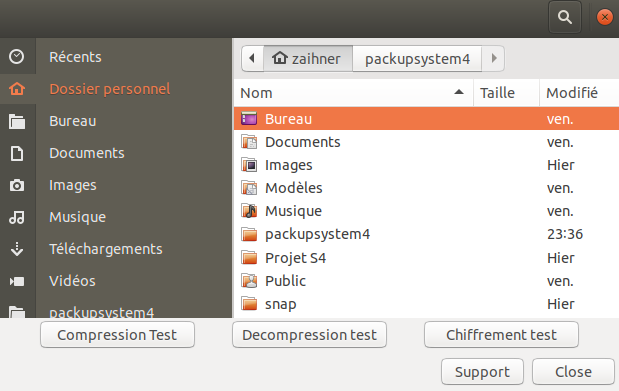
\includegraphics[width=12.1cm]{images/gui-screen.png}
		\caption{Interface actuel}
		\label{Interface actuel}
	\end{figure}
    
\newpage

\section{Site web}

    Le site web est disponible à l'adresse suivante: \url{https://packup.hyperion.tf/}. \\
    Il est actuellement hébergé sur un VPS\footnote{VPS (Virtual Private Server) = Serveur privé virtuel} d'OVH déjà utilisé par Hyperion pour herbergé plusieurs sites web. Ce serveur était idéal car il possède une configuration opérationnelle. Notre choix pour les parties de back-end et de front-end ont été très largement influencé par les infrastructure web déjà en place. Ainsi, nous avons choisit le framework Django \url{https://www.djangoproject.com/} pour le site web qui fait appel au serveur d'application uwsgi et au reverse proxy nginx.
    Pour le style et l'affichage, nous utilisons le framework Materialize (\url{https://materializecss.com/}) afin de vous présenter un site web clair et responsive.

    Pour la prochaine soutenance, nous prévoyons de créer le système d'authentification. \\
    
    \begin{figure}[!h]
		\centering
		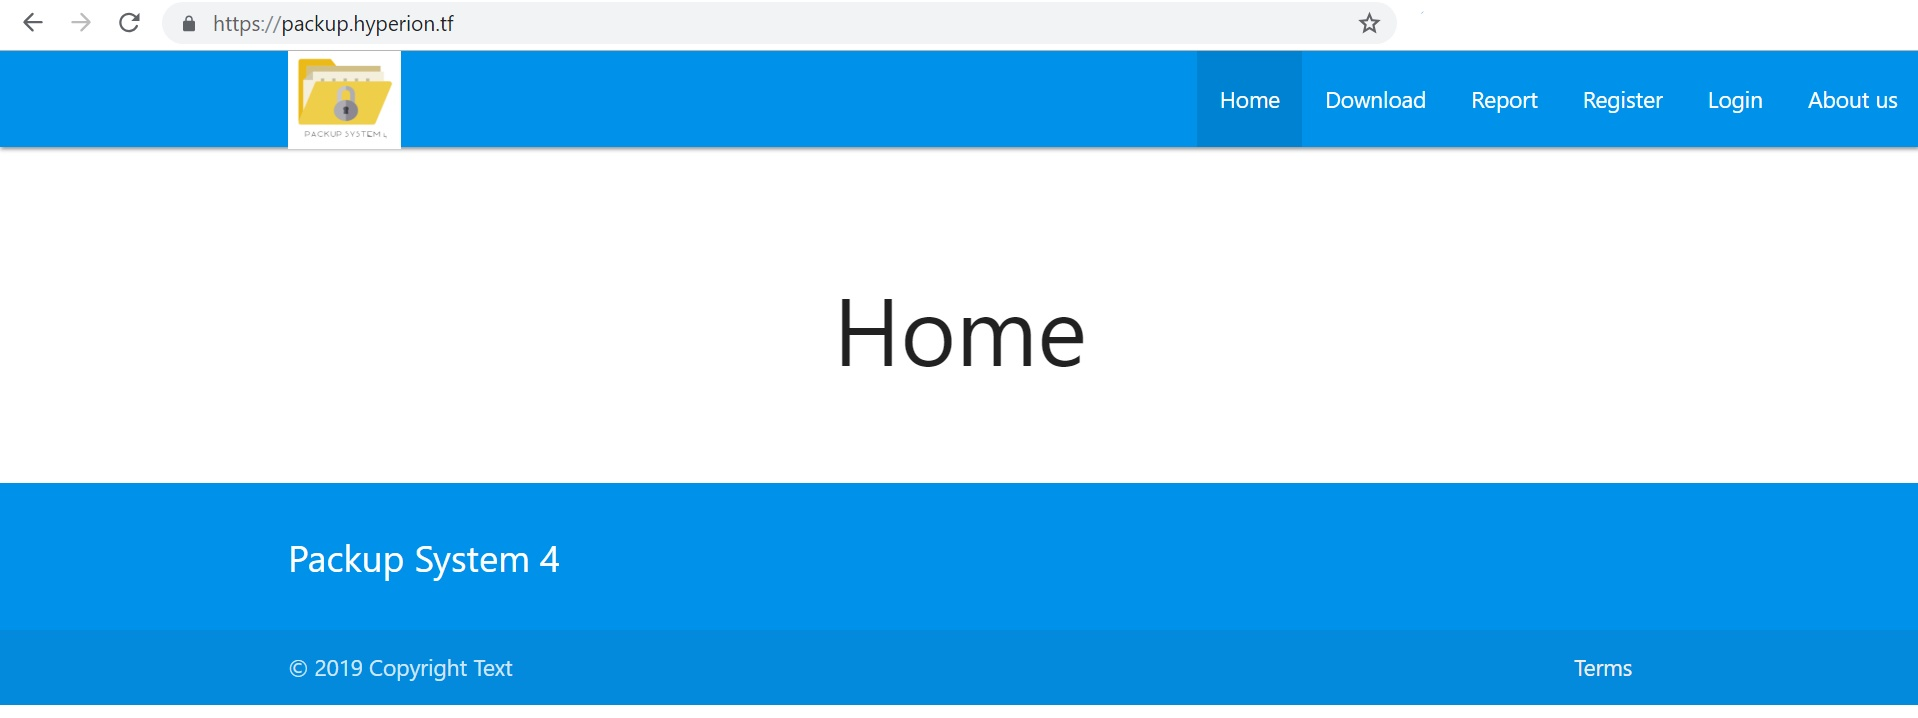
\includegraphics[width=12.5cm]{images/website.jpg}
		\caption{Site web actuel}
		\label{Site web actuel}
	\end{figure}

\newpage

\section{Avancement prévu pour les prochaines soutenances}
        
        Voici un tableau d'avancement des tâches prévu pour les prochaines soutenances : \\ \\
    
        {\normalsize
    	\begin{tabular}{|p{7.6cm}|p{1.8cm}|p{1.8cm}|p{1.8cm}|}
    		\hline
    		Tâches & \multicolumn{3}{|c|}{Soutenance} \\ 
    		\cline{2-4}
    			& \no 1 & \no 2 & \no 3 \\
    		\hline
    		Système de fichier & 75\% & 100\% & 100\% \\
    		\hline
    		Sauvegarde & 50\% & 75\% & 100\% \\
    		\hline
    		Compression & 30\% & 60\% & 100\% \\
    		\hline
    		Chiffrement & 30\% & 80\% & 100\% \\
    		\hline
    		Site web & 50\% & 80\% & 100\% \\
    		\hline
    		Interface graphique & 25\% & 60\% & 100\% \\
    		\hline
    	\end{tabular}
    	\label{répartition}}